%% LyX 2.1.4 created this file.  For more info, see http://www.lyx.org/.
%% Do not edit unless you really know what you are doing.
\documentclass[12pt,english]{report}
\usepackage{charter}
\renewcommand{\familydefault}{\rmdefault}
\usepackage[T1]{fontenc}
\usepackage[a4paper]{geometry}
\geometry{verbose,tmargin=2.5cm,bmargin=2.5cm,rmargin=2.5cm}
\setcounter{secnumdepth}{3}
\setcounter{tocdepth}{3}
\setlength{\parskip}{\medskipamount}
\setlength{\parindent}{0pt}
\usepackage{color}
\usepackage{babel}
\makeatletter

\makeatother
\usepackage{float}
\usepackage{graphicx}
\usepackage{setspace}
\usepackage{nomencl}
% the following is useful when we have the old nomencl.sty package
\providecommand{\printnomenclature}{\printglossary}
\providecommand{\makenomenclature}{\makeglossary}
\makenomenclature
\onehalfspacing
\usepackage[unicode=true,
 bookmarks=true,bookmarksnumbered=true,bookmarksopen=true,bookmarksopenlevel=1,
 breaklinks=true,pdfborder={0 0 1},backref=false,colorlinks=true]
 {hyperref}
\hypersetup{
 linkcolor=black, citecolor=red, urlcolor=blue, filecolor=blue, pdfstartview=XYZ}

\makeatletter

%%%%%%%%%%%%%%%%%%%%%%%%%%%%%% LyX specific LaTeX commands.
%% Because html converters don't know tabularnewline
\providecommand{\tabularnewline}{\\}

%%%%%%%%%%%%%%%%%%%%%%%%%%%%%% User specified LaTeX commands.
% the pages of the TOC is numbered roman
% and a pdf-bookmark for the TOC is added
\pagenumbering{roman}

%\let\myTOC\tableofcontents
%\renewcommand\tableofcontents{%
 % \pdfbookmark[1]{\contentsname}{}
 % \myTOC
 % \cleardoublepage  }

%*****Chapter style******
\usepackage[Glenn]{fncychap}
\ChNameVar{\large}
\ChTitleAsIs
\ChTitleVar{\bfseries\Huge}

%*****Header style*******
\usepackage{fancyhdr}
 
\pagestyle{fancy}

\fancyhf{}
\fancyhead[LE,RO]{\thepage}
\fancyhead[RE,LO]{\footnotesize\nouppercase{\leftmark}}

%\renewcommand{\chaptermark}[1]{\markboth{#1}{}}

\renewcommand{\headrulewidth}{0,5pt}

%****Glossaire Title*****
\renewcommand{\nomname}{Glossaire}

\makeatother

\begin{document}
\noindent 
\begin{titlepage}
\begin{center}
% Upper part of the page
\begin{minipage}{0.4\textwidth}    \end{minipage}
\begin{minipage}{0.4\textwidth} \begin{flushright} Academic year : 2018-2019 \end{flushright}\end{minipage}
\rule[0.5ex]{1\columnwidth}{1pt}\\[0.5cm]
\textsc{\large{University of Sousse}}\\
\textsc{\large{National School of Engineering of Sousse}}\\
%
\includegraphics[width=0.3\textwidth]{logo.png}\\[-0.5cm]
\Large{Graduation project report}\\[0.5cm]
\Large{ \bfseries{Applied Computer Engineering}}\\
\normalsize{Option: Distributed Systems}\\
~\\[0.6cm]
\rule[0.5ex]{1\columnwidth}{1pt}\\[0.5cm]
{ \huge \bfseries Designing and Developing a platform of remote and communicating equipements }\\[0.5cm]
\rule[0.5ex]{1\columnwidth}{1pt}\\[2cm]
% Author and supervisor
\center By: Ismail Mekni\\~\\
\newcommand\tab[1][1cm]{\hspace*{#1}}

%President	 	: 	Mr. Imed Bennour, ENISO\\
%Member 			: 	Mr. Naoufel Khayati, ENISO\\
Company supervisor	:	 Mr. Sabri Mtibaa, Sofrecom Tunisia\\
University supervisor 	:	Mr. Aref Meddeb, ENISO\\

\vfill
% Bottom of the page 
\end{center}
\end{titlepage}


\newpage
~\\
~\\
~\\
~\\
\begin{center}
To my family and all my beloved.
\end{center}



\chapter*{Acknowledgements}

IIn conducting this report, I have received meaningful assistance from many quarters which I like to put on record here with deep gratitude and great pleasure.
First and foremost, I express my sincere gratitude to my supervisors, Mr. Sabri Mtibaa, Ms. Marwa Drissi, and Mr. Aref Meddeb who extended their complete support and helped to make me deliver my best. I would also like to thank all of my teachers at the National Engineering School of Sousse for their continuous help and treasurable training during our study years. 
Finally, special thanks to the jury members who honored us by examining and evaluating this modest contribution.



\tableofcontents{}

\listoffigures


\listoftables



\chapter*{Abstract}
This report describes the design and the development of our graduation project internship, which is carried out at Sofrecom Tunisia, the project consists in creating a remote and communicating devices platform to achieve broadband supervision and monitoring and assess the quality of service “QoS” of fixed network access.
With our solution, the user could manage connected probes and create broadband tests configuration before running them in the probes, also he could manage statistics configuration with attractive charts for testing results. Users could create customized alerts configuration to simplify broadband supervision. The project also helps network supervisors to get accurate statistics according to a time period and zone area.



\section*{Keywords}
Probe – Spring boot – Angular – Raspberry Pi – Java – Kafka – Broadband – Quality of experience



\pagenumbering{arabic} 

\chapter*{General introduction}
With the global spread of the internet nowadays, many mobile and internet services operators appear. In the coming days, connected devices will spread massively worldwide, especially with the appearance of new technologies such as the internet of things, big data, personal area networks (PAN), artificial intelligence (AI). So mobile and internet services operators desire to achieve a better quality of service for their customers. To do so, operators design and develop solutions for broadband monitoring and supervision mainly to massively assess and monitor the quality of service of networks access perceived by customers. Sofrecom Tunisia, subsidiary of Orange Group, attempts to serve this purpose by designing and developing a platform for broadband supervision and monitoring and specific to massively assess the quality of service (QoS) of fixed network access. In this context comes our mission during the graduation project internship.

This report contains four chapters as follows:

The first chapter titled “Project context” will be devoted to the company presentation and setting the project in its general context.

The second chapter “Requirements analysis and specification” will be about the global system analysis to design and develop.

The third chapter “Design of the physical and logical architectures” will be dedicated to present physical and the logical architectures of our solution, also, we will explain the theory behind the broadband monitoring and supervision.

At last but not least, the final chapter “Project achievements” will be about the application achievements. First, we will present the developing environments and technologies and tools, secondly, we will illustrate our application with several interfaces.

Finally, we will close the report with a general conclusion, future work and perspectives will be mentioned at last to illustrate some ideas to improve our solution.

\chapter{Project Context}
\section{Introduction}

In the first place, this chapter will be about the host company Sofrecom Tunisia presentation, a consulting and engineering firm specializing in telecommunications. Then, we will talk about the work and the project environments, by putting the light on the project goals and the analysis of the state of the art. Finally, we will present our software development methodology and the modeling language that we are going to use.

\section{Host company presentation}


Sofrecom, a subsidiary of Orange Group, has built up 50 years’ worth of unique know-how in the telecoms operator line of business, making it a world leader in telecom consultancy and engineering. Sofrecom Tunisia is the youngest subsidiary of Sofrecom. Launched in November 2011, Sofrecom Tunisia expands Sofrecom’s presence in North Africa and the Middle East region to meet the growing demand for dedicated solutions and to offer its customers adapted and competitive offers.

\section{Project presentation}
\subsection{Problem statement}
Operators of mobile and internet services have probes, Key Performance Indicators (KPIs), installed in several network elements, but they desire to appreciate the quality perceived by their customers (Quality of Experience, QoE) in order to improve their network performance and reliability. 

In order to get accurate information about the quality of experience we should get the measurements according to zone area and specific periods of time. Also, it is difficult to manage the configuration and QoS/QoE tests running in the widespread probes, which indicates a lack of flexibility. The internet usage is improving fast; therefore we should improve the quality of service measuring as well.


\subsection{Project objectives}
This work will be considered as a graduation project to obtain applied computer science diploma from the national engineering school of Sousse (ENISO).

The main project goal is to design and develop a platform for remote and communicating devices, to serve broadband monitoring and supervision. The application should satisfy these needs:
\begin{itemize}
\item The creation and interpretation of messages exchanged with terminals and embedded equipment.
\item Information exchanges with client applications (northbound interface).
\item Management of messages from terminals (southbound interface).
\item Sending requests and messages to the terminals.
\item On-the-fly supervision of exchanges.
\item Management of supervised elements.
\item Resolution of message referral rules.
\end{itemize}

\section{Critical analysis of the state of the art}
This step is essential to propose our solution in the relation to those offered by other companies. To do so, we have studied the characteristics and the features of some available apps while we focus on their weak points.

\subsection{State of the art}
\subsubsection{SamKnows One}
The SamKnows One is a cloud-based analytics platform that includes a full range of measurement agents for fixed and cellular internet connection with a global test infrastructure. The SamKnows solution stores and visualizes performance data in real-time. This solution is implemented by a UK company “Sam” founded in 2008 by Sam Crawford. SamKnows One has developed a suite of tests as follows:
\begin{itemize}
\item	Speed tests: includes download and upload over TCP and UDP speed tests.
\item	Latency, loss and jitter: latency, jitter and packet loss 	over UDP, latency over HTML5.
\item	DNS resolution: DNS resolution time and failure rate (UDP).
\item	Web browsing: web browsing test over TCP.
\item	CDN performance: content delivery network (CDN) measurements over TCP.
\item	Video streaming: video streaming measurements that stream real content from major video streaming providers.
\item	Gaming: measures performance for a number of major games.
\item	Online storage: tests upload and download from popular online storage services.
\item	Voice over IP: measures the quality of a voice call between client and test server.
\item	Traceroute: tests the path that traffic takes around the internet, it is useful in diagnosing routing issues.
\item	Data usage: measures of data used on the broadband connection.
\end{itemize}


\begin{figure}[H]
\centering
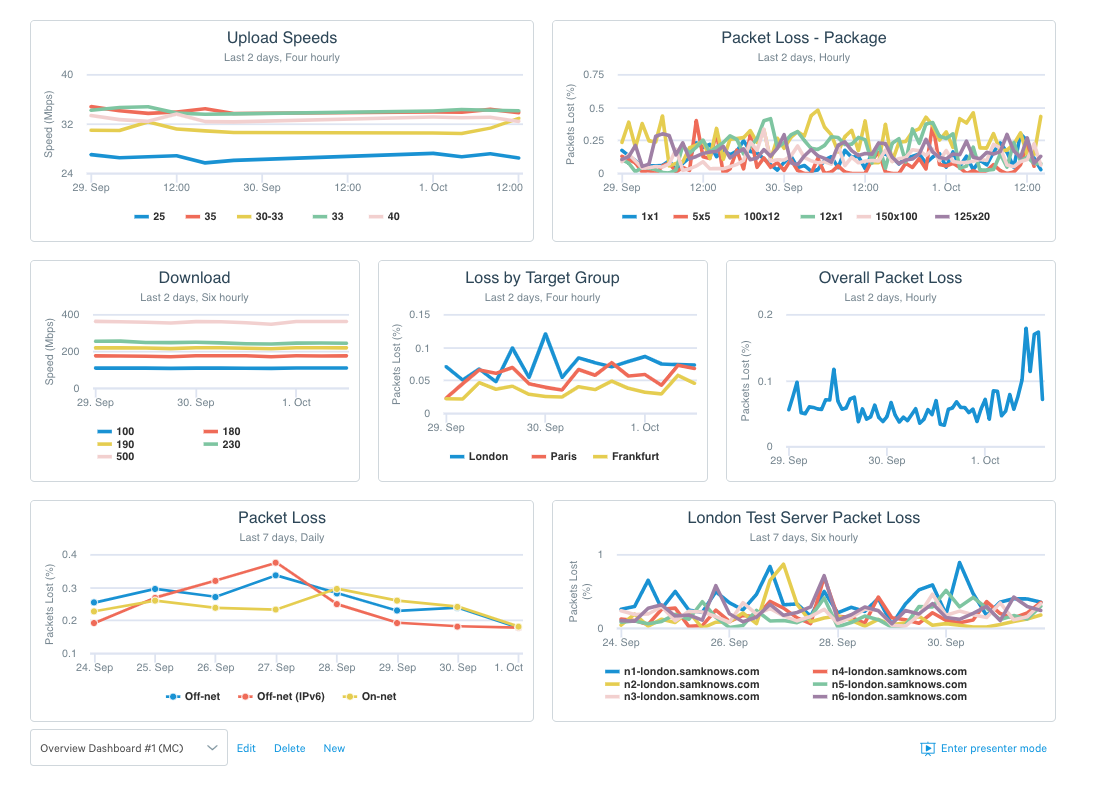
\includegraphics[width=15cm]{samknows.png}
\caption{Screenshot of SamKnows One dashboard}
\label{fig:samknows}
\end{figure}

\subsubsection{SMAQ}
SMAQ is a solution implemented by Sofrecom to generate reports and analysis based upon different broadband tests, this solution is used by the Orient Middle East and Africa Orange affiliates. 

\begin{figure}[H]
\centering
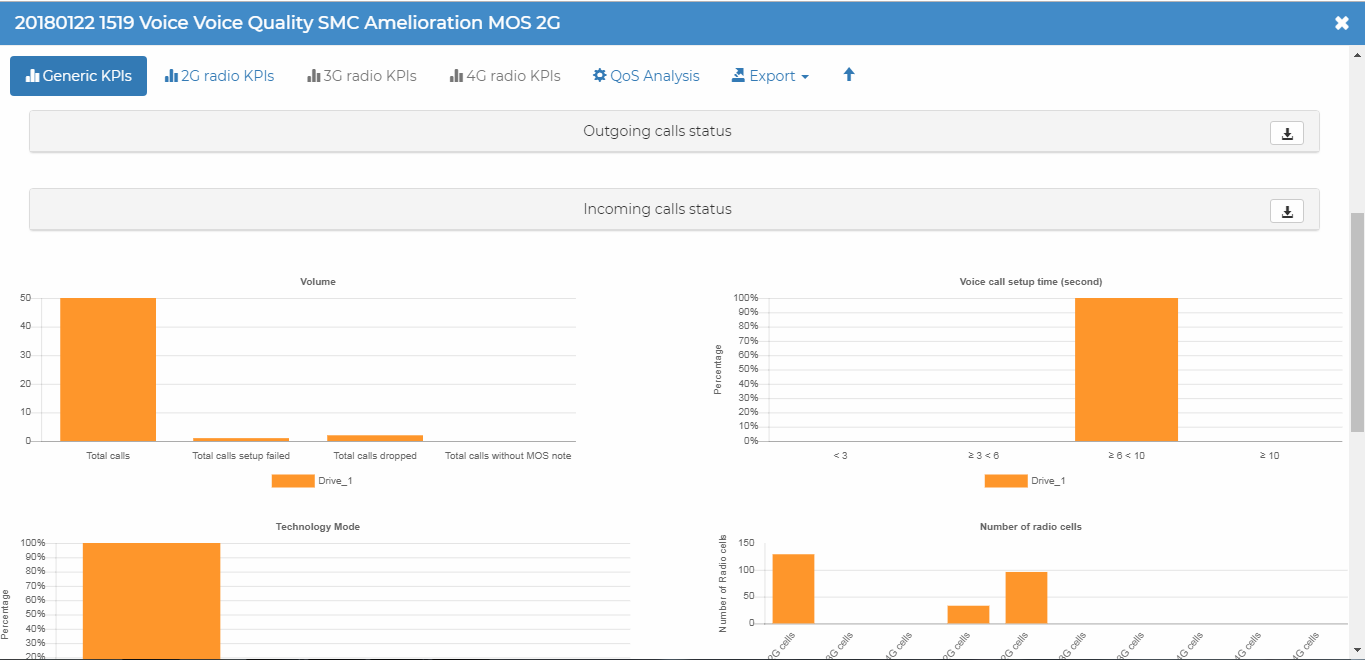
\includegraphics[width=15cm]{smaq.png}
\caption{Screenshot of SMAQ online dashboard}
\label{fig:smaq}
\end{figure}


\subsection{Critical of the state of the art}
The following table shows in detail the difference between the two mentioned solutions:
\begin{table}[H]
\centering
\begin{tabular}{|l|l|l|l|l|l|}
\hline
Solution                       & SamKnows One & SMAQ \\ \hline
Paying solution                      & YES         & NO \\ \hline
Analytics                 & YES         & YES \\ \hline
Custom dashboard & YES         & NO \\ \hline
Mapping data                 & YES         & NO  \\ \hline
Generate reports                    & YES         & YES  \\ \hline
Network monitoring (alerting)                    & YES         & YES \\ \hline
Users management              & YES          & NO \\ \hline
Devices management              & NO          & NO \\ \hline
Tests management              & NO          & NO \\ \hline
\end{tabular}
\caption{Comparison of state of the art}
\label{my-label}
\end{table}


Sofrecom Tunisia is looking for an open source solution for the issue in question so SamKnows One solution is not convenient for them, in the other hand SMAQ provides just the basic functionalities. The weak point in the mentioned solutions, they don’t give users the access to devices configuration. Network supervisors can’t customize tests to satisfy their specific needs.

\subsection{Proposed solution:}
The solution proposed by Sofrecom Tunisia is to design and develop a platform for broadband monitoring and supervision, “SMAQ Probes”, the solution should respond the following needs:

\begin{itemize}
\item	Online device management and task scheduling.
\item	Online test management.
\item	Online statistics and customized charts configuration.
\item	Online alerts configuration and customization.
\item	Online user management.
\end{itemize}

\section{Modeling language}
During the work on our solution we used UML “Unified Modeling Language” for describing and modeling the specifications of our project. UML is a flexible and versatile modeling language, also it is the most popular and widely used by the community. We are going to present some diagrams from UML that we find it useful during our work:

\begin{itemize}
\item	Use case diagram: it helps to structure the needs of users and the corresponding objectives of our system by identifying its users and their interactions.
\item	Sequence diagram: it is a time focus representation of objects and their interactions.
\item	Package diagram: it gives an overview of the application packages. It is a high abstraction that presents the application modularity.
\item	Class diagram: it gives a presentation of classes and interfaces of our system and relations between them.
\item	Activity diagram: it gives an overview of the dynamic aspects of the system.
\end{itemize}

\section{Software development methodology}
Before starting the project design and development, we should choose appropriate software development methodology to work with. The software development methodology helps to describe the different phases and the sequences of application development process.

During our project, we used agile kanban because it is a most convenient method to us. I am the only intern working on the project. Changes in the project can happen any time. We are continuously improving the flow of work. We are trying to limit work in progress and to maximize efficiency. Also, we focus on reducing the time it takes to take a project from start to finish.


\section{Conclusion}

In this chapter, we presented the general context of the project by presenting the host company Sofrecom Tunisia, the problem statement and the state of the art.

In the next chapter, we will model the requirements of our solution through use case diagrams.

\chapter{Requirements Analysis and Specification}

\section{Introduction}

The requirements analysis and specification phase is an essential step for the development of a new application. It allows presenting the application’s features in detail.

In this chapter, the first part will be devoted to identify the different actors of the application who are interacting with the system and to give the functional and nonfunctional requirements definitions. Subsequently, we will present the general system analysis using use case diagrams.

\section{Identification of the actors:}
An actor is an abstraction of a role of actual user who is in a perpetual interaction with the application. Following on, our system’s actor along with his role and granted permissions.

\subsection*{Internal actors}

\begin{itemize}
\item	Application administrator: the administrator is responsible of managing users and their permission, he has the permission to create, read, update, and delete users. Also, he has the permission to check all the other configurations like devices configuration and test configuration.
\item	Network supervisor: the network supervisor has the permission to read the different configurations without editing them. He has the right to supervise the quality of experience “QOS”.
\item	Network and broadband administrator: he has all the rights of the network supervisor, in addition, he has the permission to create, read, update, and delete broadband monitoring configurations.
\end{itemize}

\subsection*{External actors}

\begin{itemize}
\item	Probe: the probe is the entity able to get devices and tests configuration, and send the metrics to the server after running tests.
\end{itemize}

\section{Functional requirements}

Functional requirements refer to primary functions that each component of our solution must exhibit. It is a set of services which are:
\subsection*{For the web application}

\begin{itemize}
\item	The application should give the administrator the hand to manage users’ accounts.
\item	The application should give permitted users the possibility to customize their dashboards.
\item	The application should give permitted users the access to manage the network monitoring (alerting).
\item	The application should provide permitted users with the access to tests and devices configurations.
\item	The application should be able to process received metrics data in real-time.
\end{itemize}

\subsection*{For the hardware}

\begin{itemize}
\item	The boards should be able to receive and implement their configurations in real-time.
\item	The boards should be able to run tests according to the time scheduler and send results to the server.
\item	The boards should be able to send their current configuration (location, IP address, device identifier, jobs configuration).
\item	The boards should be able to keep the tests results if the server is not available.
\end{itemize}

\section{Non-functional requirements}
Non-functional requirements refer to several key features that are beyond the purpose of the solution, they specify criteria that judge the operation of a system, rather than specific behaviors in order to ensure the client’s satisfaction.
\paragraph{Extensibility}
~\\
The system must be open to some extension like for example adding new features if needed without radical modification in the code.
\paragraph{Performance}
~\\
The web application should be as efficient as possible with especially a good response time. Users should be able to receive the quality of experience (QOE) from the cloud server within a reasonable amount of time.
\paragraph{Re-usability}
~\\
The system shouldn’t be exclusive for our case and must be adaptive to other use cases.
\paragraph{Robustness}
~\\
The system must cope with errors during execution and should be able to reboot within a short time in case of failure.
\paragraph{Security}
~\\
The user’s personal information must be kept safe from others and only system administrator has permissions to access it. The broadband monitoring and supervision access must be permitted to the supervisors of the network in question.

\section{Requirements analysis}
On one hand, this section offers a better understanding of the mentioned requirements by declaring them in a semi-formal way. On the other hand, it emphasizes the interactions between the actor and our application. In contemplation of breaking down the complexity of these goals, we use the use case diagrams. 

\begin{figure}[H]
\centering
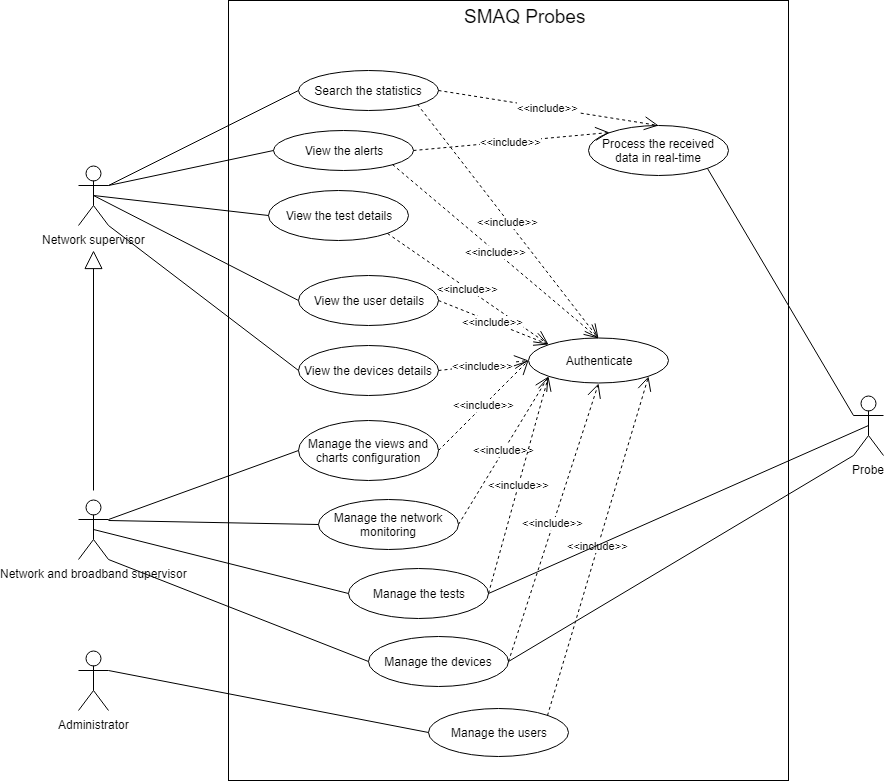
\includegraphics[width=15cm,height=16cm]{general-use-case-diagram.png}
\caption{General use case diagram}
\label{fig:usecasegeneral}
\end{figure}

As shown in the general use case diagram (fig.\ref{fig:usecasegeneral}), only the administrator can register all types of users. All the features of the application must go through authentication. The network and broadband supervisor is responsible for managing network monitoring, devices configuration, tests, and statistics configuration. Any configuration that concerns probes configuration will be sent to probes. Probes send their information and runs tests according to a job scheduler, then probes send tests results to the server, thus, our system process the received data in real-time. Finally our system is prepared to generate statistics and quality of service for the network supervisor.

\subsection{Manage devices}

\begin{figure}[H]
\centering
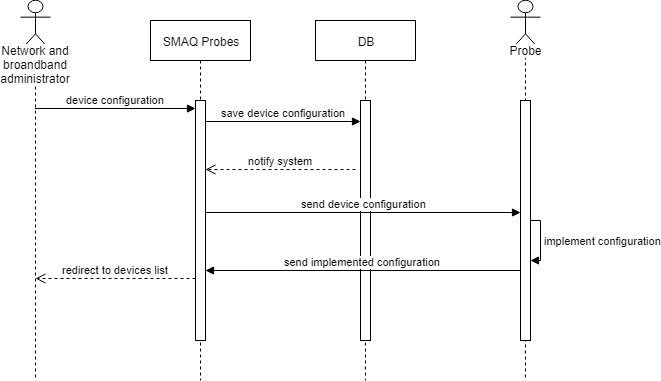
\includegraphics[width=15cm, height=14cm]{manage-device-sequece-diagram.png}
\caption{Devices management sequence diagram}
\label{fig:devicesequence}
\end{figure}

\begin{table}[H]
\centering
\begin{tabular}{|l|l|}
\hline
Title             & Device management                                                                                                                                                                                                                                                                                    \\ \hline
Author            & Ismail MEKNI                                                                                                                                                                                                                                                                             \\ \hline
Version           & 1.0                                                                                                                                                                                                                                                                                             \\ \hline
Objectives        & Allow users to manage connected devices configuration
 \\ \hline
Actors            & \begin{tabular}[c]{@{}l@{}}Network and broadband administrator – SMAQ Probes – \\Probe\end{tabular}                                                                                                                                                                                                                                                                                                                                                                                                                                                                                                                                                                                                                                                                                                          \\ \hline
Pre-conditions    & \begin{tabular}[c]{@{}l@{}}The user should authenticate as network and broadband\\ administrator.\\ The device should be connected.\end{tabular}                                                                                                                                                                  \\ \hline
Post-conditions   & \begin{tabular}[c]{@{}l@{}}New device configuration is persisted in the database.\\ New device configuration is implemented in the probe.\end{tabular}                                                                                                                                                                                                                                                                                                                                                                                                                             \\ \hline
Story             & \begin{tabular}[c]{@{}l@{}}1. The user enters device new configuration (status, \\IP address, client name, job scheduling).\\ 2. The user submits the changes.\end{tabular}                                                                                    \\ \hline
Alternative story & \begin{tabular}[c]{@{}l@{}}\end{tabular}                                                                                                                                                                            \\ \hline
Exceptional story & \begin{tabular}[c]{@{}l@{}}The device in question is not connected; the configuration’s\\ message will be suspended waiting the device to reconnect.\end{tabular} \\ \hline
\end{tabular}
\caption{Device management description}
\label{my-label}
\end{table}

As shown in the devices management sequence diagram (fig.\ref{fig:devicesequence}), the device management functionality is permitted to network and broadband administrators. User can access to the devices list. User can select a device to edit its configuration (IP address, location, registered client name, job scheduling), if user submits the new configuration, the configuration will be sent to the backend system to persist it to database. Also the configuration will be sent to the device in question, the probe, device, implements the changes. Finally, the probe sends back the implemented configurations to the system as a confirmation.

\subsection{Manage tests}

\begin{figure}[H]
\centering
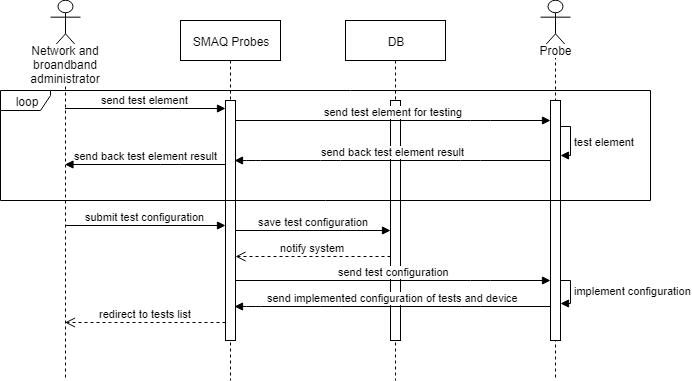
\includegraphics[width=15cm, height=14cm]{tests-management-sequence-diagram.png}
\caption{Tests management sequence diagram}
\label{fig:testsequence}
\end{figure}

\begin{table}[H]
\centering
\begin{tabular}{|l|l|}
\hline
Title             & Tests management                                                                                                                                                                                                                                                                                    \\ \hline
Author            & Ismail MEKNI                                                                                                                                                                                                                                                                             \\ \hline
Version           & 1.0                                                                                                                                                                                                                                                                                             \\ \hline
Objectives        & Allow users to manage tests configuration.
 \\ \hline
Actors            & \begin{tabular}[c]{@{}l@{}}Network and broadband administrator – SMAQ Probes – \\Probe\end{tabular}
\\ \hline
Pre-conditions    & \begin{tabular}[c]{@{}l@{}}The user should authenticate as network and broadband \\administrator.\\ At least one device should be connected.\end{tabular}                                                                                                                                                                  \\ \hline
Post-conditions   & \begin{tabular}[c]{@{}l@{}}New tests configuration is persisted in the database.\\ New tests are running on the probes.\end{tabular}                                                                                                                                                                                                                                                                                                                                                                                                                             \\ \hline
Story             & \begin{tabular}[c]{@{}l@{}}1. The user tests each element directly on the device.\\ 2. The user submits the test configuration with all elements.\end{tabular}                                                                                    \\ \hline
Alternative story & \begin{tabular}[c]{@{}l@{}}\end{tabular}                                                                                                                                                                            \\ \hline
Exceptional story & \begin{tabular}[c]{@{}l@{}}There is no connected device, so user can’t test elements,\\ the operation with be suspended until at least one device\\ reconnect.\end{tabular} \\ \hline
\end{tabular}
\caption{Test management description}
\label{my-label}
\end{table}

As shown above in the diagram (fig.\ref{fig:testsequence}), the access to the test configuration is granted to users with network and broadband administrator role. To edit test configuration, user should enter test elements, each element must be tested directly on the probe, device, and then test’s element result will be sent back to the user. After creating and testing all the elements, a new test configuration will be sent to the backend system. The configuration is persisted to database. The new test configuration is sent to the probes, all the probes implement the new test configuration. Finally a signal messages is sent from all the probes holding the current configurations.

\subsection{Manage network monitoring}

\begin{figure}[H]
\centering
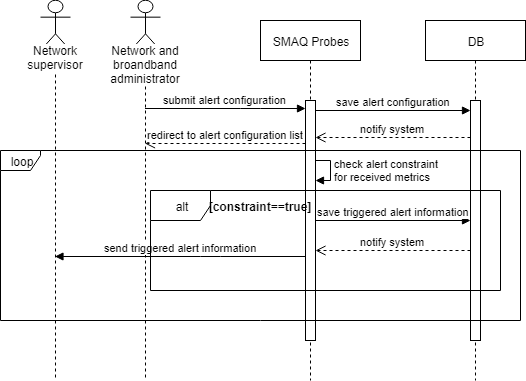
\includegraphics[width=15cm, height=14cm]{network-monitoring-management-sequence-diagram.png}
\caption{Network monitoring management sequence diagram}
\label{fig:monitoringsequence}
\end{figure}

\begin{table}[H]
\centering
\begin{tabular}{|l|l|}
\hline
Title             & Network monitoring management
\\ \hline
Author            & Ismail MEKNI                                                                                                                                                                                                                                                                             \\ \hline
Version           & 1.0                                                                                                                                                                                                                                                                                             \\ \hline
Objectives        & \begin{tabular}[c]{@{}l@{}} Allow users to manage network monitoring configuration,\\ alerting system.\end{tabular}
 \\ \hline
Actors            & \begin{tabular}[c]{@{}l@{}}Network and broadband administrator – Network supervisor\\ – SMAQ Probes\end{tabular}
\\ \hline
Pre-conditions    & \begin{tabular}[c]{@{}l@{}}The user should authenticate as network and broadband \\administrator to access the network monitoring management.\\ To view triggered alerts, the user should authenticate as a\\ network supervisor.\end{tabular}                                                                                                                                                                  \\ \hline
Post-conditions   & \begin{tabular}[c]{@{}l@{}}New alert configuration is persisted in the database.\\ Alert listener is running on the received metrics.\end{tabular}                                                                                                                                                                                                                                                                                                                                                                                                                             \\ \hline
Story             & \begin{tabular}[c]{@{}l@{}}1. The user send alert configuration containing the constraint.\\ 2. The network supervisor can view alerts if triggered.\end{tabular}                                                                                    \\ \hline
Alternative story & \begin{tabular}[c]{@{}l@{}}\end{tabular}                                                                                                                                                                            \\ \hline
Exceptional story & \begin{tabular}[c]{@{}l@{}}\end{tabular} \\ \hline
\end{tabular}
\caption{Network monitoring management description}
\label{my-label}
\end{table}

As shown in the diagram (fig.\ref{fig:monitoringsequence}), the user authenticates with network and broadband administrator. This feature aims to configure customized alerts. User creates alerts with a specific constraint. This configuration will be persisted to database. An alert checker will be run for every received metrics data, if the constraint is satisfied an alert with full description will be triggered. The triggered alerts are persisted to database so network supervisors can check them.

\subsection{Manage statistics and charts configuration}

\begin{figure}[H]
\centering
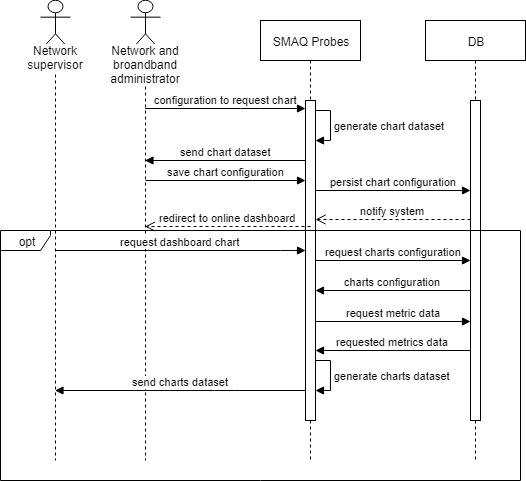
\includegraphics[width=15cm, height=14cm]{charts-management-sequence-diagram.png}
\caption{Charts management sequence diagram}
\label{fig:chartssequence}
\end{figure}

\begin{table}[H]
\centering
\begin{tabular}{|l|l|}
\hline
Title             & Charts and statistics management
\\ \hline
Author            & Ismail MEKNI                                                                                                                                                                                                                                                                             \\ \hline
Version           & 1.0                                                                                                                                                                                                                                                                                             \\ \hline
Objectives        & Allow users to manage charts configuration.
 \\ \hline
Actors            & \begin{tabular}[c]{@{}l@{}}Network and broadband administrator – Network supervisor\\ – SMAQ Probes\end{tabular}
\\ \hline
Pre-conditions    & \begin{tabular}[c]{@{}l@{}}The user should authenticate as network and broadband \\administrator to access charts and statistics management.\\ To view dashboard, the user should authenticate as a \\network supervisor.\end{tabular}                                                                                                                                                                  \\ \hline
Post-conditions   & \begin{tabular}[c]{@{}l@{}}New chart configuration is persisted in the database.\\ New chart is added to dashboard.\end{tabular}                                                                                                                                                                                                                                                                                                                                                                                                                             \\ \hline
Story             & \begin{tabular}[c]{@{}l@{}}1. The user send chart configuration, system generates chart \\dataset.\\ 2. Chart displayed to user.\\ 3. User submit chart configuration.\end{tabular}                                                                                    \\ \hline
Alternative story & \begin{tabular}[c]{@{}l@{}}\end{tabular}                                                                                                                                                                            \\ \hline
Exceptional story & \begin{tabular}[c]{@{}l@{}}\end{tabular} \\ \hline
\end{tabular}
\caption{Charts management description}
\label{my-label}
\end{table}

As we can see in the above sequence diagram (fig.\ref{fig:chartssequence}), to access to charts and statistics configuration, users should have network and broadband administrator privileges. User enters the chart parameters; our system generates the chart in question. User submits this configuration to be persisted and added to dashboard. Thus, users with network supervisor permission can see the configured charts on the dashboard. This feature aims to allow users to create customized charts and views.

\subsection{Manage users}

\begin{figure}[H]
\centering
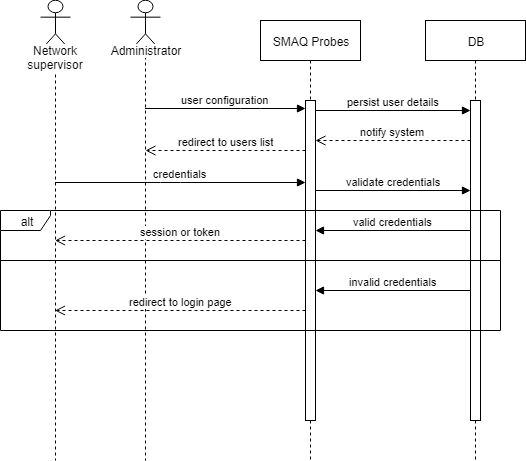
\includegraphics[width=15cm, height=14cm]{users-management-sequence-diagram.png}
\caption{Users’ management sequence diagram}
\label{fig:userssequence}
\end{figure}

\begin{table}[H]
\centering
\begin{tabular}{|l|l|}
\hline
Title             & Users management
\\ \hline
Author            & Ismail MEKNI                                                                                                                                                                                                                                                                             \\ \hline
Version           & 1.0                                                                                                                                                                                                                                                                                             \\ \hline
Objectives        & \begin{tabular}[c]{@{}l@{}}Allow administrator to manage users’ configuration and \\details.\end{tabular}
 \\ \hline
Actors            & \begin{tabular}[c]{@{}l@{}}Administrator – Network supervisor – SMAQ Probes\end{tabular}
\\ \hline
Pre-conditions    & \begin{tabular}[c]{@{}l@{}}The user should authenticate as application administrator to \\access the users’ management.\end{tabular}                                                                                                                                                                  \\ \hline
Post-conditions   & \begin{tabular}[c]{@{}l@{}}User credential is persisted to database.\\User can authenticate.\end{tabular}                                                                                                                                                                                                                                                                                                                                                                                                                             \\ \hline
Story             & \begin{tabular}[c]{@{}l@{}}1. The administrator submit user configuration.\\ 2. The user submits his credentials.\end{tabular}                                                                                   
 \\ \hline
Alternative story & \begin{tabular}[c]{@{}l@{}}\end{tabular}                                                                                                                                                                            \\ \hline
Exceptional story & \begin{tabular}[c]{@{}l@{}}If the user enters invalid credentials, he will be prompted to \\try to login again.\end{tabular} \\ \hline
\end{tabular}
\caption{Users management description}
\label{my-label}
\end{table}

As shown in the users' management sequence diagram (fig.\ref{fig:userssequence}), the users’ management feature is only allowed to the application administrator. The administrator enters the credentials of each user. Thus, user is now registered to the application and he can access to the application features according to his privileges. To sign in to the application, the user enters his credentials, generally a username and a password, if the credentials are valid, he will be redirected to the dashboard, and else he will be prompted to login again. 

\section{Conclusion}

Throughout this chapter, we specified and analyzed the requirements that solution should deliver to users, and we presented the main scenarios and the use cases that it should offer.

The next chapter aims to go a step further in the process of developing the application via presenting the design of the different components of our system.


\chapter{Design of the Physical and Logical Architectures}

\section{Introduction}
\section{Physical architecture}
\section{Logical architecture}
\subsection{Conceptual model}
\subsection{Modular decomposition}
\subsection{Broadband supervision and monitoring theory}
\section{Conclusion}

\chapter{Project Achievements}

\section{Introduction}
\section{Developing environment}
\subsection{Hardware envionment}
\subsection{Software environment}
\subsection{Frameworks and technologies}
\section{Achieved work}
\subsection{Authentication and users management}
\subsection{Devices management}
\subsection{Metrics and tests management}
\subsection{Statistics and dashboard management}
\subsection{Alerts management}
\section{Conclusion}
\chapter{General Conclusion and Future Work}


\begin{thebibliography}{9}


\end{thebibliography}

\chapter*{Appendix}

\end{document}
